% !TeX encoding=utf8
% !TeX spellcheck = en-US

\chapter{Publications}
%\markboth{Publications}{Publications}

The following publications of mine formed the basis of this thesis.

%% In these lists the publications are numbered by date of publications
%% and the author of the thesis can be printed in bold.


% \section*{Wissenschaftliche Veröffentlichungen}
\begin{refsection}
\nocite{Halchenko2021, wagner2020datalad, wagner2022fairly}
% NISO2022119623, HankePestilliWagnerMarkiewiczPolineHalchenko+2021+17+25,
\begin{refcontext}[sorting=nyt]  
	\printbibliography[heading=none, resetnumbers=true]
\end{refcontext}
%\end{refsection}

My contributions to these works are as follows:

For \citet{wagner2020datalad}, I conceived the conceptual structure and educational concept, co-created the technical backbone, coordinated development efforts and community management, and wrote most of its contents.\\
For \citet{Halchenko2021}, I contributed to the conceptualization, writing, and editing of the manuscript, and have been a regular contributor to the underlying software since 2019.\\
For \citet{wagner2022fairly}, I co-conceived the setup of the framework, co-piloted and documented an earlier version of the framework with a smaller dataset, co-implemented the open workflow, wrote the first draft of the manuscript, and contributed to the conceptualization, writing, and editing of the manuscript.

The original publications from \citet{Halchenko2021} and \citet{wagner2022fairly} are included hereafter.

% \section*{Beiträge auf internationalen Konferenzen}
%\begin{refsection}
%\nocite{wagner202310, wagnerohbm2022, wagnerohbm2021, poldrackohbm2020, wagner_adina_s_2020_7906718}

%\printbibliography[env=numbered+bold, heading=none, sorting=ynt, resetnumbers=true]
%\begin{refcontext}[sorting=nyt]
%	\printbibliography[heading=none, resetnumbers=true]
%\end{refcontext}
%\end{refsection}

% \section*{Beiträge auf nationalen Konferenzen}
%\begin{refsection}
%\nocite{adina_s_wagner_2021_4541323}

%\printbibliography[env=numbered+bold, heading=none, sorting=ynt, resetnumbers=true]
%\begin{refcontext}[sorting=nyt]
%	\printbibliography[heading=none, resetnumbers=true]
%\end{refcontext}


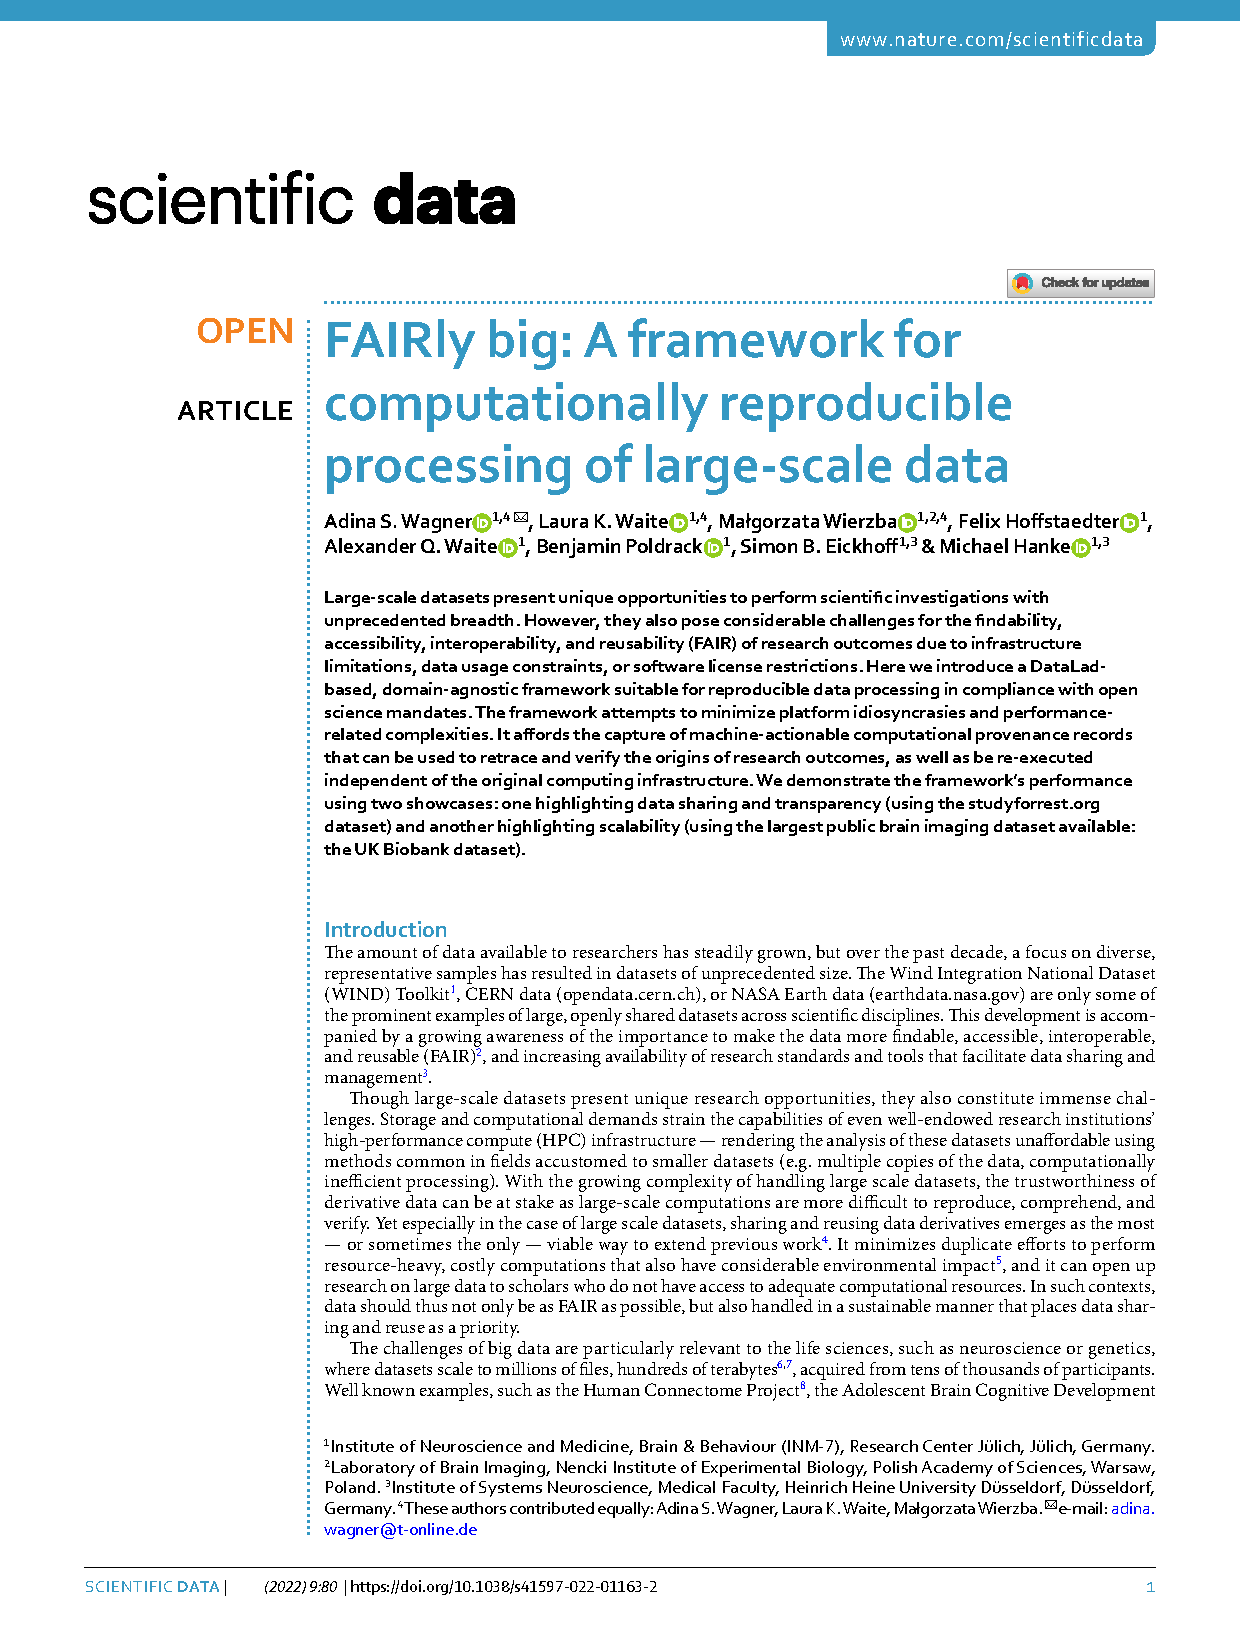
\includepdf[pages=1-17]{content/appendix_pub_fairlybig.pdf}
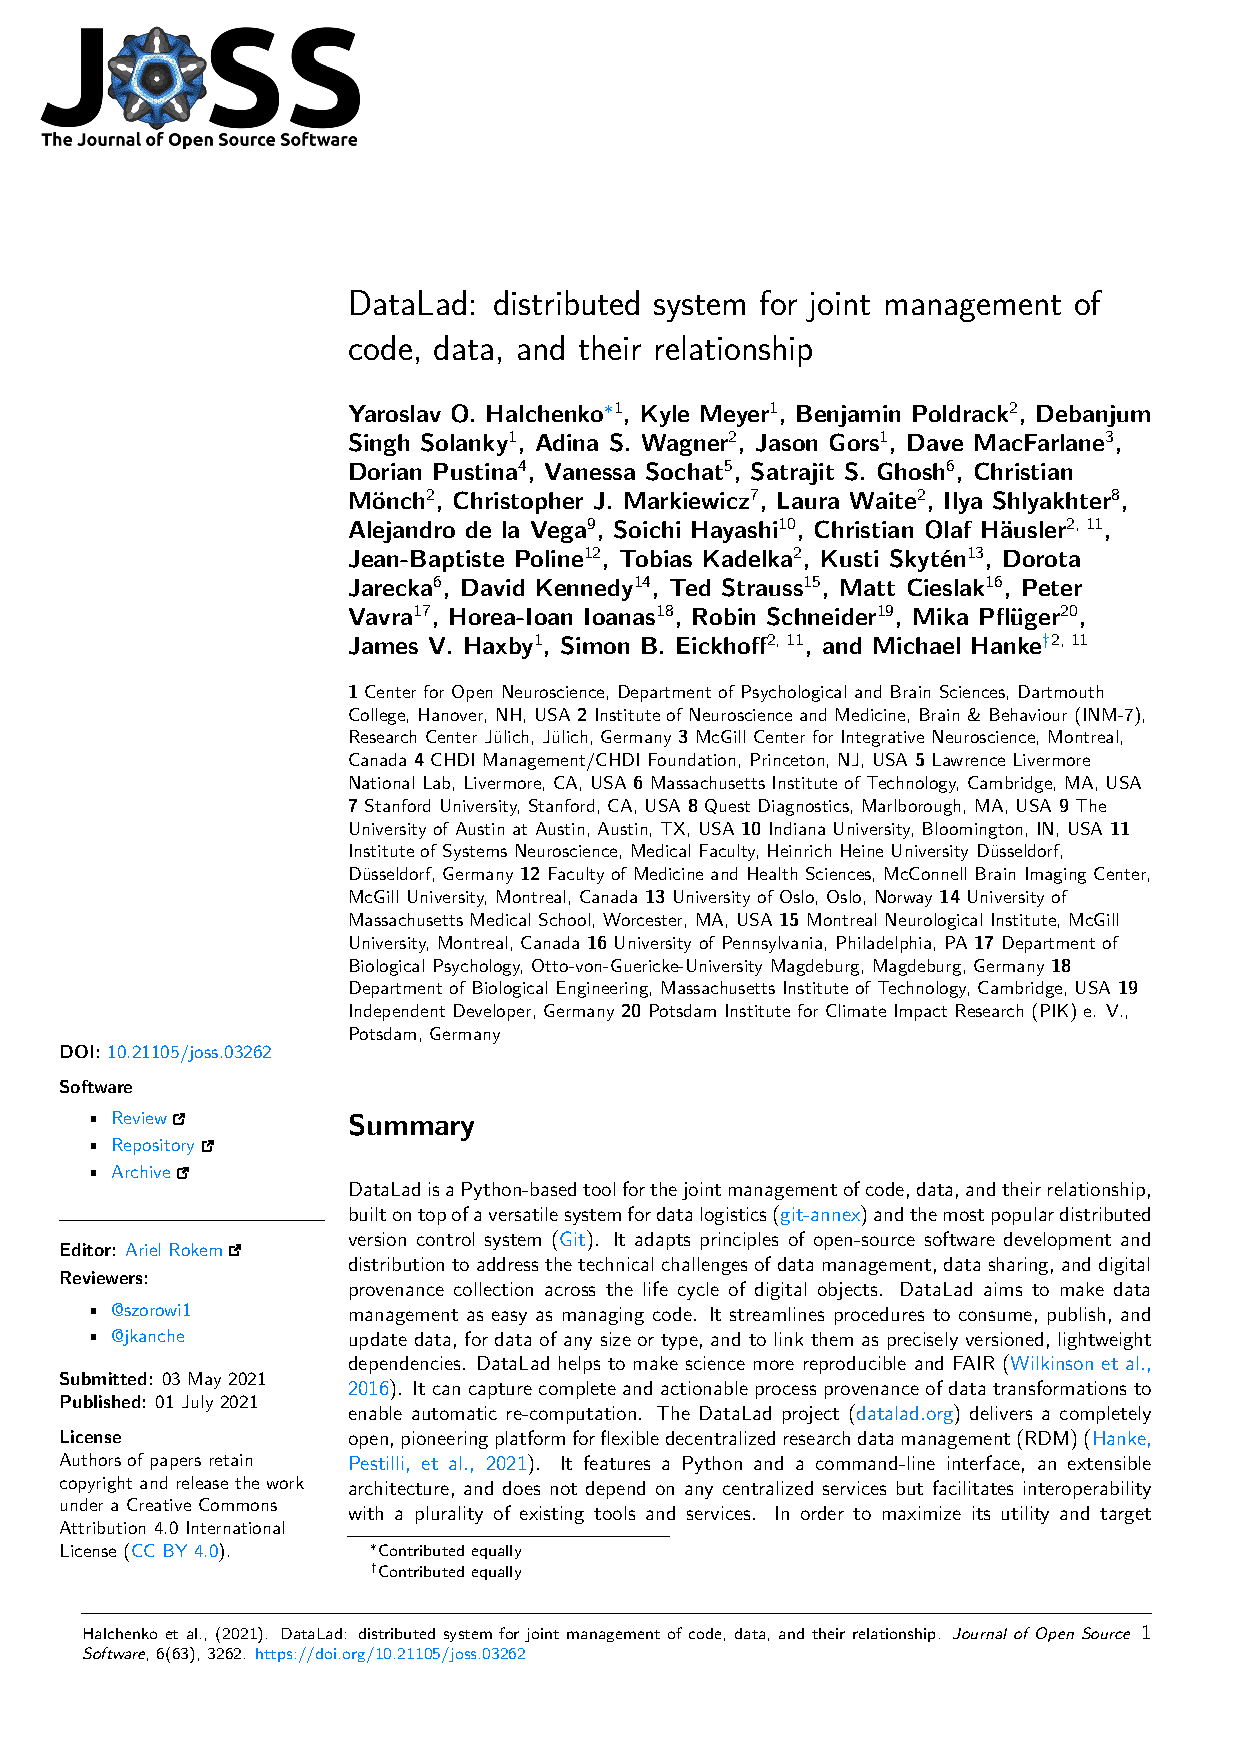
\includepdf[pages=1-8]{content/appendix_pub_datalad.pdf}

\end{refsection}
%
